\documentclass[10pt,a4paper]{article}

\usepackage[utf8]{inputenc}
\usepackage[T1]{fontenc}
\usepackage{lmodern}
\usepackage[a4paper,top=1.8cm,bottom=1.8cm,left=1.8cm,right=1.8cm]{geometry}
\usepackage{xcolor}
\usepackage{tikz}
\usetikzlibrary{calc,shapes.geometric,backgrounds}
\usepackage{booktabs}
\usepackage{tabularx}
\usepackage{enumitem}
\usepackage{titlesec}
\usepackage{fancyhdr}
\usepackage{microtype}
\usepackage[colorlinks=true,linkcolor=primary,urlcolor=secondary]{hyperref}

% =========================================================
% Color Palette
% =========================================================
\definecolor{primary}{RGB}{30, 58, 138}        % Deep navy blue
\definecolor{secondary}{RGB}{2, 132, 199}      % Cyan/Sky blue
\definecolor{darkslate}{RGB}{51, 65, 85}       % Slate grey
\definecolor{bordergray}{RGB}{209, 213, 219}   % Light grey border
\definecolor{boxbg}{RGB}{248, 250, 252}        % Light subtle card bg

% Terminal Colors (Light Grey Theme)
\definecolor{termbg}{RGB}{246, 248, 250}       % Light grey background
\definecolor{termbar}{RGB}{229, 231, 235}      % Slightly darker grey title bar
\definecolor{termborder}{RGB}{209, 213, 219}   % Border grey
\definecolor{termtext}{RGB}{31, 41, 55}        % Dark charcoal text
\definecolor{termuser}{RGB}{22, 101, 52}       % Dark green for user
\definecolor{termhost}{RGB}{21, 128, 61}       % Green for host
\definecolor{termpath}{RGB}{29, 78, 216}       % Blue for directory path
\definecolor{termcmd}{RGB}{17, 24, 39}         % Bold black for commands
\definecolor{termout}{RGB}{55, 65, 81}         % Clear dark grey for outputs
\definecolor{termdir}{RGB}{37, 99, 235}        % Blue for directories
\definecolor{termfile}{RGB}{31, 41, 55}        % Dark for regular files
\definecolor{termhidden}{RGB}{107, 114, 128}   % Muted grey for hidden files
\definecolor{termsize}{RGB}{180, 83, 9}        % Amber for sizes
\definecolor{termperm}{RGB}{79, 70, 229}       % Indigo for permissions

% =========================================================
% Section Headings (Clean, No Underline)
% =========================================================
\titleformat{\section}
  {\color{primary}\large\bfseries\sffamily}
  {\thesection.}{0.5em}{}
\titlespacing*{\section}{0pt}{8pt}{3pt}

\titleformat{\subsection}
  {\color{secondary}\normalsize\bfseries\sffamily}
  {\thesubsection}{0.5em}{}
\titlespacing*{\subsection}{0pt}{6pt}{2pt}

% =========================================================
% Headers and Footers (Completely Clean Footers)
% =========================================================
\pagestyle{fancy}
\fancyhf{}
\renewcommand{\headrulewidth}{0.4pt}
\renewcommand{\footrulewidth}{0pt}
\fancyhead[L]{\small\sffamily\color{darkslate} Operating Systems Lab}
\fancyhead[R]{\small\sffamily\color{darkslate} Lab Report: Linux File Management}
\fancyfoot{}

% First page style: no header at top, no footer at bottom
\fancypagestyle{firstpage}{%
  \fancyhf{}
  \renewcommand{\headrulewidth}{0pt}
  \renewcommand{\footrulewidth}{0pt}
}

% =========================================================
% Terminal Window Macro (Light Grey with Crisp Edges)
% =========================================================
\newcommand{\termprompt}[1][\textasciitilde]{%
  \textbf{\textcolor{termuser}{ratul}}\textcolor{termtext}{@}\textbf{\textcolor{termhost}{firefly}}\textcolor{termtext}{:}\textbf{\textcolor{termpath}{#1}}\textcolor{termcmd}{\$}\ %
}

\newcommand{\terminalwindow}[3][\linewidth]{%
\begin{center}
\begin{tikzpicture}
  % 1. Terminal text on main layer
  \node[
      text=termtext,
      font=\ttfamily\fontsize{7.2}{9.2}\selectfont,
      align=left,
      text width=\dimexpr#1-0.95cm\relax,
      inner xsep=7pt,
      inner ysep=7pt,
      anchor=north west
  ] (body) at (0.32cm, -0.56cm) {#3};

  % Coordinates
  \coordinate (topleft) at (0, 0);
  \coordinate (bottomright) at ($(body.south -| #1, 0) + (0, -6pt)$);
  \coordinate (titlecenter) at ($0.5*(topleft) + 0.5*(#1, 0) + (0, -0.28cm)$);

  % 2. Background and Title bar on background layer
  \begin{scope}[on background layer]
    % Light grey terminal body
    \fill[termbg, rounded corners=6pt] (topleft) rectangle (bottomright);

    % Title bar (clipped to match rounded top corners)
    \begin{scope}
      \clip[rounded corners=6pt] (topleft) rectangle (bottomright);
      \fill[termbar] (topleft) rectangle (#1, -0.56cm);
      \draw[termborder, line width=0.5pt] (0, -0.56cm) -- (#1, -0.56cm);
    \end{scope}

    % Continuous outer border (smooth, no distortion)
    \draw[termborder, line width=0.6pt, rounded corners=6pt] (topleft) rectangle (bottomright);
  \end{scope}

  % 3. Window control dots
  \fill[red!80!black] (0.36cm, -0.28cm) circle (0.07cm);
  \fill[yellow!80!black] (0.63cm, -0.28cm) circle (0.07cm);
  \fill[green!75!black] (0.90cm, -0.28cm) circle (0.07cm);

  % 4. Centered terminal title
  \node[
      text=gray!40!black,
      font=\sffamily\bfseries\fontsize{7.2}{8}\selectfont,
      anchor=center
  ] at (titlecenter) {#2};
\end{tikzpicture}
\end{center}
\vspace{-6pt}
}

\newcommand{\cmd}[1]{\texttt{\textbf{#1}}}

\begin{document}
\thispagestyle{firstpage}

% =========================================================
% Title: Only Experiment Title at the Top
% =========================================================
\begin{center}
  {\Large\bfseries\sffamily\color{primary} Experiment Title: File and Directory Management in Linux Terminal}\\[3pt]
  {\normalsize\sffamily\textbf{Topic:} Creating, Copying, Moving, and Removing Files and Directories}
\end{center}
\vspace{-4pt}

% =========================================================
% 1. Objective
% =========================================================
\section{Objective}
The objective of this lab is to learn how to create, duplicate, relocate, and delete files and directories using the Linux command-line interface. By completing this experiment, we aim to:
\begin{itemize}[noitemsep,topsep=1pt,leftmargin=1.2em]
  \item Create single and nested folders using \cmd{mkdir} and \cmd{mkdir -p}.
  \item Create new empty files quickly using the \cmd{touch} command.
  \item Duplicate files into new locations or new names using \cmd{cp}.
  \item Move files between folders and rename existing files using \cmd{mv}.
  \item Safely delete files and directories using \cmd{rm}, \cmd{rm -r}, and \cmd{rm -rf}.
\end{itemize}

% =========================================================
% 2. Equipment / Software Requirements
% =========================================================
\section{Equipment / Software Requirements}
\vspace{-2pt}
\begin{table}[h!]
\centering\footnotesize
\renewcommand{\arraystretch}{1.08}
\begin{tabularx}{\linewidth}{lXlX}
\toprule
\textbf{Item} & \textbf{Details} & \textbf{Item} & \textbf{Details} \\
\midrule
\textbf{Operating System} & Linux (NixOS 26.11, Kernel 6.12) & \textbf{Host Machine} & \texttt{firefly} \\
\textbf{User Account} & \texttt{ratul} & \textbf{Command Shell} & GNU Bash 5.2 / Zsh \\
\textbf{Terminal Emulator} & Linux Terminal (Kitty / Ghostty) & \textbf{Core Tools} & GNU Coreutils (\texttt{mkdir}, \texttt{touch}, \texttt{cp}, \texttt{mv}, \texttt{rm}) \\
\bottomrule
\end{tabularx}
\end{table}
\vspace{-8pt}

% =========================================================
% 3. Theoretical Background
% =========================================================
\section{Theoretical Background}
File and directory management is the most essential skill in Linux. Unlike graphical file managers where users click and drag icons, the terminal allows us to organize, copy, and clean up files very quickly using short commands.

\subsection{Commands Practiced in This Lab}
\vspace{-2pt}
\begin{table}[h!]
\centering\footnotesize
\renewcommand{\arraystretch}{1.08}
\begin{tabularx}{\linewidth}{llp{5.5cm}X}
\toprule
\textbf{Command} & \textbf{Syntax} & \textbf{Simple Meaning / Purpose} & \textbf{Example} \\
\midrule
\cmd{mkdir} & \texttt{mkdir <name>} & Creates a new empty directory (folder). & \texttt{mkdir docs} \\
\cmd{mkdir -p} & \texttt{mkdir -p <path>} & Creates parent and child folders together in one step. & \texttt{mkdir -p proj/src/utils} \\
\cmd{touch} & \texttt{touch <file>} & Creates a new empty file, or updates timestamp. & \texttt{touch notes.txt} \\
\cmd{cp} & \texttt{cp <src> <dest>} & Copies a file to a new name or destination folder. & \texttt{cp notes.txt backup.txt} \\
\cmd{mv} & \texttt{mv <src> <dest>} & Moves a file to another folder, or renames it. & \texttt{mv old.txt new.txt} \\
\cmd{rm} & \texttt{rm <file>} & Deletes one or more files permanently. & \texttt{rm temp.log} \\
\cmd{rm -r} & \texttt{rm -r <folder>} & Deletes a folder and all its contents recursively. & \texttt{rm -r old\_data} \\
\cmd{rm -rf} & \texttt{rm -rf <path>} & Forcefully deletes folder and files without any prompt. & \texttt{rm -rf build} \\
\bottomrule
\end{tabularx}
\end{table}
\vspace{-6pt}

\subsection{Important Rules for File Operations}
\begin{itemize}[noitemsep,topsep=1pt,leftmargin=1.2em]
  \item \textbf{No Recycle Bin in Terminal:} Commands like \cmd{rm} delete files immediately and permanently. There is no graphical Trash folder to recover deleted files.
  \item \textbf{Parent Flag (\cmd{-p}):} Standard \cmd{mkdir a/b/c} fails if folder \cmd{a} does not exist yet. Adding \cmd{-p} tells Linux to build all missing parent folders automatically.
  \item \textbf{Recursive Flag (\cmd{-r}):} Standard \cmd{rm} refuses to remove directories. The \cmd{-r} (recursive) flag dives inside the directory and removes all files and subfolders first.
  \item \textbf{Force Flag (\cmd{-f}):} Suppresses all warning messages and ignores non-existent files. Combined as \cmd{rm -rf}, it forces complete removal without stopping.
\end{itemize}

\newpage

% =========================================================
% 4. Demo Directory Structure
% =========================================================
\section{Equipment / Demo Directory Setup}
To practice these commands safely, we created an isolated practice folder called \cmd{lab3\_demo} inside \texttt{/home/ratul}. The diagram below shows the structure we constructed, organized, and cleaned during this lab:

\begin{center}
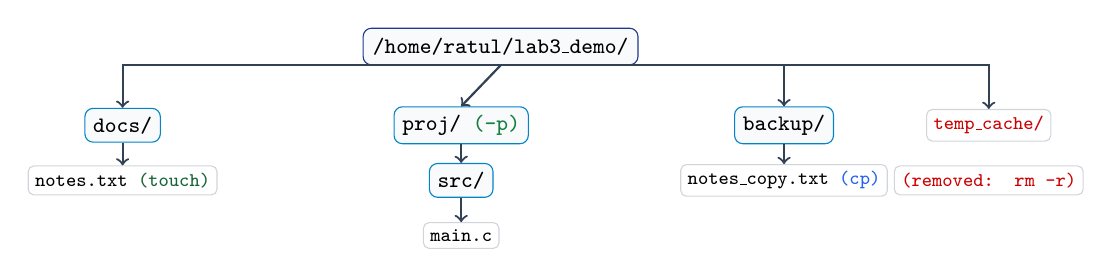
\begin{tikzpicture}[
  x=1cm, y=1cm,
  dirbox/.style={draw=primary, fill=boxbg, rounded corners=3pt, font=\ttfamily\footnotesize\bfseries, inner sep=3.5pt},
  subbox/.style={draw=secondary, fill=boxbg, rounded corners=3pt, font=\ttfamily\footnotesize\bfseries, inner sep=3pt},
  filebox/.style={draw=bordergray, fill=white, rounded corners=2pt, font=\ttfamily\scriptsize, inner sep=2.5pt},
  actionbox/.style={draw=bordergray, fill=white, rounded corners=2pt, font=\ttfamily\scriptsize, text=darkslate, inner sep=2.5pt}
]
  % Root node
  \node[dirbox] (root) at (0, 0) {/home/ratul/lab3\_demo/};

  % Branches
  \node[subbox] (docs)  at (-4.8, -1.0) {docs/};
  \node[filebox] (f1)   at (-4.8, -1.7) {notes.txt \textcolor{termuser}{\textbf{(touch)}}};

  \node[subbox] (proj)  at (-0.5, -1.0) {proj/ \textcolor{termhost}{\textbf{(-p)}}};
  \node[subbox] (src)   at (-0.5, -1.7) {src/};
  \node[filebox] (f2)   at (-0.5, -2.4) {main.c};

  \node[subbox] (bak)   at (3.6, -1.0) {backup/};
  \node[filebox] (f3)   at (3.6, -1.7) {notes\_copy.txt \textcolor{termdir}{\textbf{(cp)}}};

  \node[actionbox] (del) at (6.2, -1.0) {\textcolor{red!80!black}{\textbf{temp\_cache/}}};
  \node[actionbox] (del2) at (6.2, -1.7) {\textcolor{red!80!black}{\textbf{(removed: rm -r)}}};

  % Arrows
  \draw[->, thick, darkslate] (root.south) -| (docs.north);
  \draw[->, thick, darkslate] (docs.south) -- (f1.north);
  \draw[->, thick, darkslate] (root.south) -- (proj.north);
  \draw[->, thick, darkslate] (proj.south) -- (src.north);
  \draw[->, thick, darkslate] (src.south) -- (f2.north);
  \draw[->, thick, darkslate] (root.south) -| (bak.north);
  \draw[->, thick, darkslate] (bak.south) -- (f3.north);
  \draw[->, thick, darkslate] (root.south) -| (del.north);
\end{tikzpicture}
\end{center}
\vspace{-8pt}

% =========================================================
% 5. Procedure / Steps
% =========================================================
\section{Procedure / Steps}
We carried out the file and directory management tasks using the following simple steps:
\begin{enumerate}[noitemsep,topsep=1pt,leftmargin=1.4em]
  \item Created our practice workspace folder \cmd{lab3\_demo} using \cmd{mkdir} and entered it with \cmd{cd}.
  \item Created a simple directory called \cmd{docs} using \cmd{mkdir}.
  \item Created a multi-level nested folder tree \cmd{proj/src/utils} in one single command using \cmd{mkdir -p}.
  \item Created new empty text files (\cmd{notes.txt} and \cmd{main.c}) using the \cmd{touch} command.
  \item Made a backup folder and duplicated \cmd{notes.txt} into \cmd{notes\_copy.txt} using \cmd{cp}.
  \item Moved \cmd{notes\_copy.txt} into the \cmd{backup/} folder and renamed files using \cmd{mv}.
  \item Deleted a single unwanted file safely using \cmd{rm}.
  \item Created a temporary folder containing files and deleted it completely using \cmd{rm -r}.
  \item Tested forced recursive deletion of stubborn folder trees using \cmd{rm -rf}.
\end{enumerate}

% =========================================================
% 6. Result / Output Demonstration (Session 1)
% =========================================================
\section{Result / Output Demonstration}
All commands were executed under user account \texttt{ratul} on host machine \texttt{firefly}.

\subsection{Session 1: Creating Directories, Nested Trees, Empty Files, and Copying}

\terminalwindow{ratul@firefly: \textasciitilde/lab3\_demo\ \textemdash\ bash}{
% Command 1: mkdir
\termprompt[\textasciitilde/lab3\_demo]\textbf{\textcolor{termcmd}{mkdir docs backup}}

\vspace{0.08cm}
% Command 2: mkdir -p
\termprompt[\textasciitilde/lab3\_demo]\textbf{\textcolor{termcmd}{mkdir -p proj/src/utils}}

\vspace{0.08cm}
% Command 3: touch
\termprompt[\textasciitilde/lab3\_demo]\textbf{\textcolor{termcmd}{touch docs/notes.txt proj/src/main.c}}

\vspace{0.08cm}
% Command 4: ls to verify creation
\termprompt[\textasciitilde/lab3\_demo]\textbf{\textcolor{termcmd}{ls docs proj/src}}

\textcolor{termout}{docs:}\ \ \textcolor{termfile}{notes.txt}\ \ \ \ \ \ \ \ \ \ \ \ \textcolor{termout}{proj/src:}\ \ \textcolor{termfile}{main.c}\ \ \textcolor{termdir}{\textbf{utils}}

\vspace{0.14cm}
% Command 5: cp
\termprompt[\textasciitilde/lab3\_demo]\textbf{\textcolor{termcmd}{cp docs/notes.txt docs/notes\_copy.txt}}

\vspace{0.08cm}
% Command 6: ls docs
\termprompt[\textasciitilde/lab3\_demo]\textbf{\textcolor{termcmd}{ls -l docs}}

\textcolor{termout}{total 0}

\textcolor{termperm}{-rw-r--r--}\ 1\ \textcolor{termuser}{ratul}\ \textcolor{termhost}{users}\ 0\ Oct\ \ 8\ 14:10\ \textcolor{termfile}{notes.txt}

\textcolor{termperm}{-rw-r--r--}\ 1\ \textcolor{termuser}{ratul}\ \textcolor{termhost}{users}\ 0\ Oct\ \ 8\ 14:12\ \textcolor{termfile}{notes\_copy.txt}

\vspace{0.10cm}
% Active cursor
\termprompt[\textasciitilde/lab3\_demo]\textbf{\textcolor{termcmd}{\rule{0pt}{0.9em}\textunderscore}}
}

\paragraph{Explanation of Session 1 Results:}
\begin{itemize}[noitemsep,topsep=1pt,leftmargin=1.2em]
  \item \cmd{mkdir} and \cmd{mkdir -p}: Created \texttt{docs} and \texttt{backup}. With \cmd{-p}, Linux automatically created the whole chain \texttt{proj/src/utils} without complaining that parent folders were missing.
  \item \cmd{touch}: Instantly created new files \texttt{notes.txt} and \texttt{main.c} with 0 bytes size.
  \item \cmd{cp}: Duplicated \texttt{notes.txt} into \texttt{notes\_copy.txt}. Both files now exist independently in the folder.
\end{itemize}

\newpage

% =========================================================
% 6. Result / Output Demonstration (Session 2)
% =========================================================
\subsection{Session 2: Moving, Renaming, and Removing Files and Directories}

\terminalwindow{ratul@firefly: \textasciitilde/lab3\_demo\ \textemdash\ bash}{
% Command 7: mv to move
\termprompt[\textasciitilde/lab3\_demo]\textbf{\textcolor{termcmd}{mv docs/notes\_copy.txt backup/}}

\vspace{0.08cm}
% Command 8: mv to rename
\termprompt[\textasciitilde/lab3\_demo]\textbf{\textcolor{termcmd}{mv backup/notes\_copy.txt backup/notes\_v1.txt}}

\vspace{0.08cm}
% Command 9: verify mv
\termprompt[\textasciitilde/lab3\_demo]\textbf{\textcolor{termcmd}{ls backup}}

\textcolor{termfile}{notes\_v1.txt}

\vspace{0.14cm}
% Command 10: touch temporary file and delete with rm
\termprompt[\textasciitilde/lab3\_demo]\textbf{\textcolor{termcmd}{touch temp.log \&\& rm temp.log}}

\vspace{0.08cm}
% Command 11: setup folder for rm -r
\termprompt[\textasciitilde/lab3\_demo]\textbf{\textcolor{termcmd}{mkdir -p temp\_cache/data \&\& touch temp\_cache/data/cache.bin}}

\vspace{0.08cm}
% Command 12: delete with rm -r
\termprompt[\textasciitilde/lab3\_demo]\textbf{\textcolor{termcmd}{rm -r temp\_cache}}

\vspace{0.14cm}
% Command 13: test rm -rf on nested tree
\termprompt[\textasciitilde/lab3\_demo]\textbf{\textcolor{termcmd}{mkdir -p scratch/a/b \&\& touch scratch/a/test.tmp}}

\vspace{0.08cm}
% Command 14: delete with rm -rf
\termprompt[\textasciitilde/lab3\_demo]\textbf{\textcolor{termcmd}{rm -rf scratch}}

\vspace{0.08cm}
% Command 15: final verify
\termprompt[\textasciitilde/lab3\_demo]\textbf{\textcolor{termcmd}{ls}}

\textcolor{termdir}{\textbf{backup}}\ \ \ \ \textcolor{termdir}{\textbf{docs}}\ \ \ \ \textcolor{termdir}{\textbf{proj}}

\vspace{0.10cm}
% Final prompt
\termprompt[\textasciitilde/lab3\_demo]\textbf{\textcolor{termcmd}{\rule{0pt}{0.9em}\textunderscore}}
}

\paragraph{Explanation of Session 2 Results:}
\begin{itemize}[noitemsep,topsep=1pt,leftmargin=1.2em]
  \item \cmd{mv} for moving and renaming: When given a destination folder (\texttt{backup/}), \cmd{mv} relocated the file. When given a new file name (\texttt{notes\_v1.txt}), \cmd{mv} renamed the file in place.
  \item \cmd{rm}: Deleted the single file \texttt{temp.log} instantly.
  \item \cmd{rm -r}: Successfully deleted the non-empty folder \texttt{temp\_cache} by removing its subfolder and file recursively.
  \item \cmd{rm -rf}: Forcibly deleted the entire \texttt{scratch} hierarchy without asking confirmation or throwing errors.
  \item Final verification with \cmd{ls} confirmed our workspace remained clean with only \texttt{backup}, \texttt{docs}, and \texttt{proj}.
\end{itemize}

% =========================================================
% 7. Conclusion
% =========================================================
\section{Conclusion}
In this lab, we practiced the primary commands used for everyday file and directory management in Linux. We learned:
\begin{enumerate}[noitemsep,topsep=1pt,leftmargin=1.4em]
  \item How to create single folders with \cmd{mkdir} and nested folder paths with \cmd{mkdir -p}.
  \item How to generate files with \cmd{touch} and duplicate them safely using \cmd{cp}.
  \item How to relocate and rename files efficiently using the \cmd{mv} command.
  \item How to delete files with \cmd{rm}, and recursively remove directory structures using \cmd{rm -r} and \cmd{rm -rf}.
\end{enumerate}
Understanding these commands enables fast and structured organization of files in the Linux operating system.

\end{document}
